% !TEX root = Bachelorarbeit Synthetische Daten.tex
\chapter{Ergebnisse} \label{sec:results}

Dieses Kapitel präsentiert die Ergebnisse der Arbeit. Es wird auf die generierten synthetischen Daten eingegangen und die Trainings- und Testergebnisse der Modelle beschrieben. Anschließend wird die Klassifikations-Performance der Modelle verglichen und die Out-of-Distribution-Detektion analysiert.

\section{Die generierten synthetischen Daten} \label{sec:da-fusion-results}

% Einleitung/Überblick

% Validation Images; stetiges Verbessern (Gemeinsames Finetuning)
...

\subsection{In-Distribution} \label{sec:da-fusion-id-results}

% Beispiele

% Menschliche Evaluierung (eigene)
	% Größtenteils überzeugend
	% Teilweise questionable
...

\begin{figure}
	\centering
	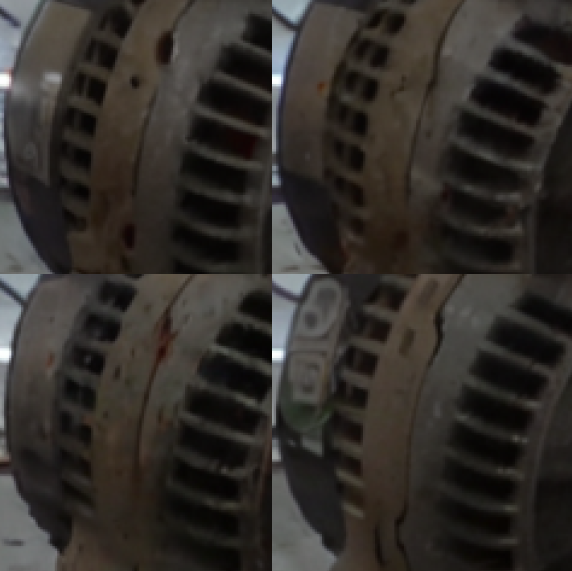
\includegraphics[width=0.5\textwidth]{figure_results_id-augs_detail_1.png}%
	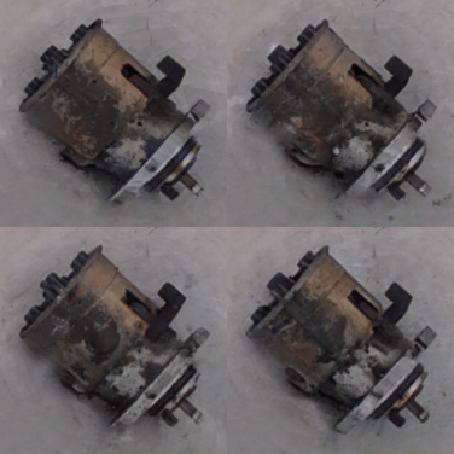
\includegraphics[width=0.5\textwidth]{figure_results_id-augs_detail_2.png}
	\caption{Vergrößerte Ausschnitte der synthetischen In-Distribution-Daten.}
	\label{fig:id-augs-detail}
\end{figure}

\subsection{Near Out-of-Distribution} \label{sec:da-fusion-ood-results}

% Beispiele

% Menschliche Evaluierung (eigene)
...

\section{Trainings- und Testergebnisse} \label{sec:supcon-results}

...

\subsection{Contrastive Pre-Training} \label{sec:supcon-pre-results}

% Nur reale Daten
% Mit ID-Augmentationen
% Mit ID-Augmentationen und OOD-Augmentationen für hard-negative mining
...

\begin{figure}
	\centering
	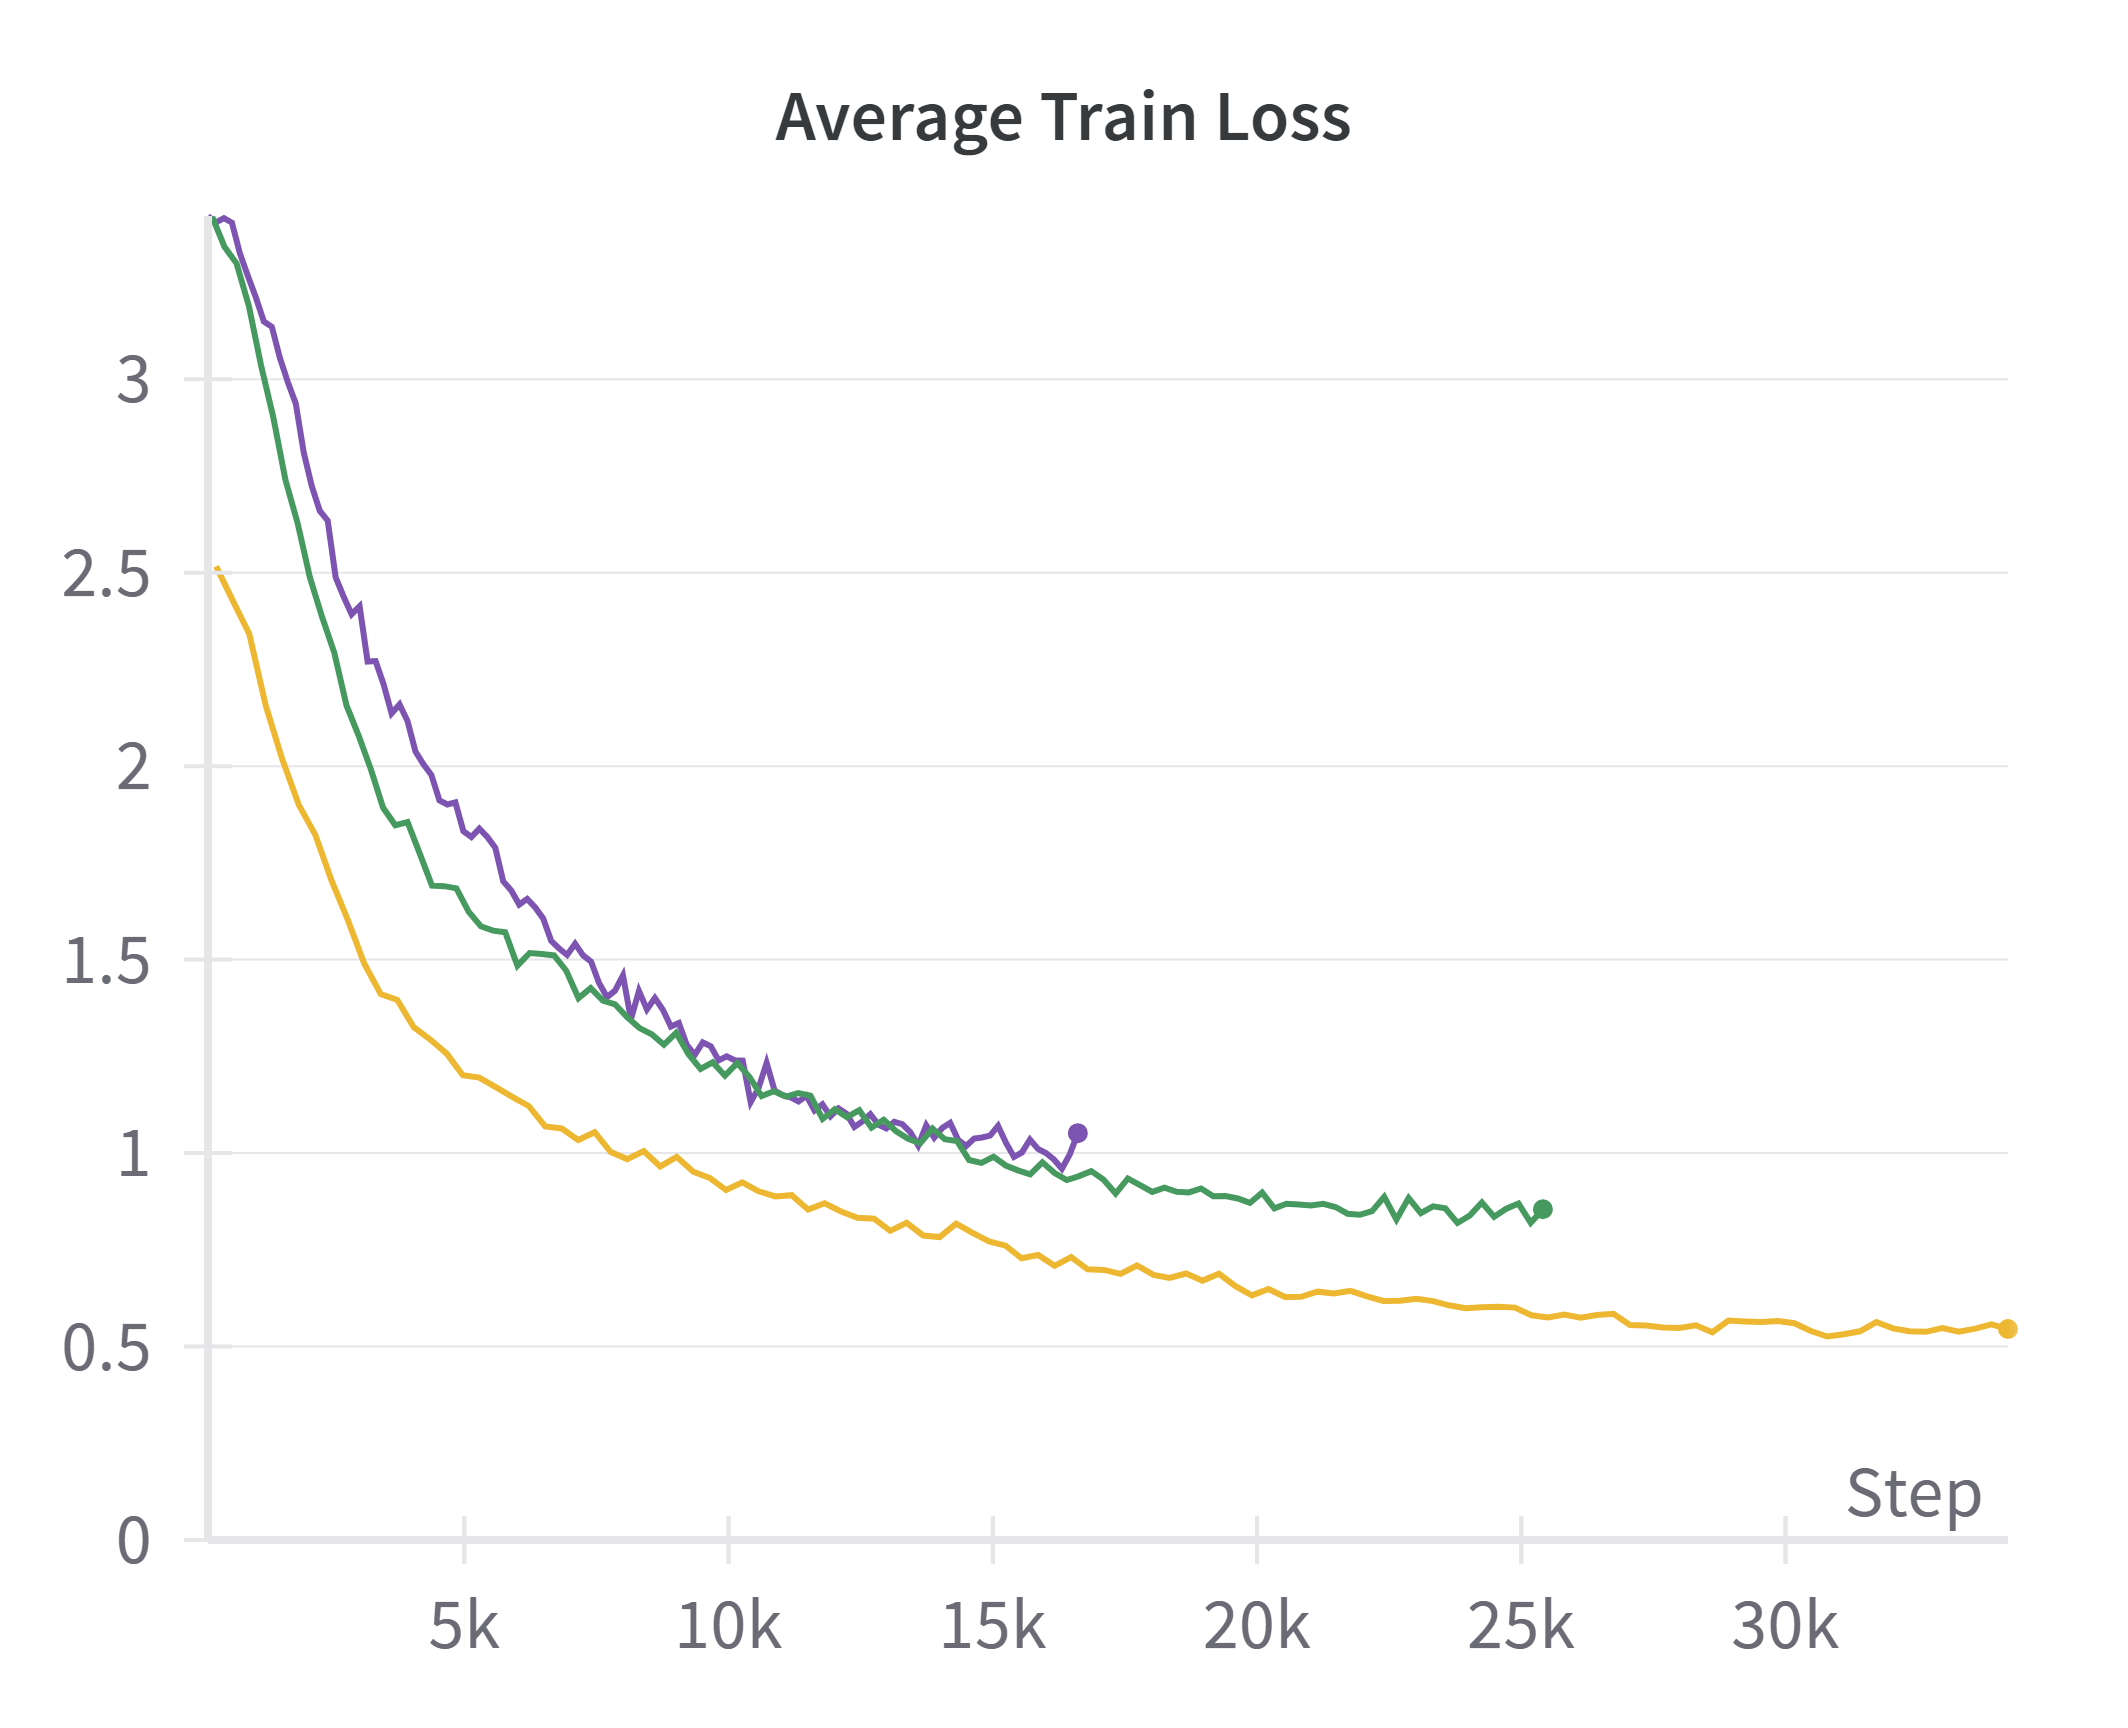
\includegraphics[width=0.5\textwidth]{figure_results_supcon-pre_avg-train-loss.png}%
	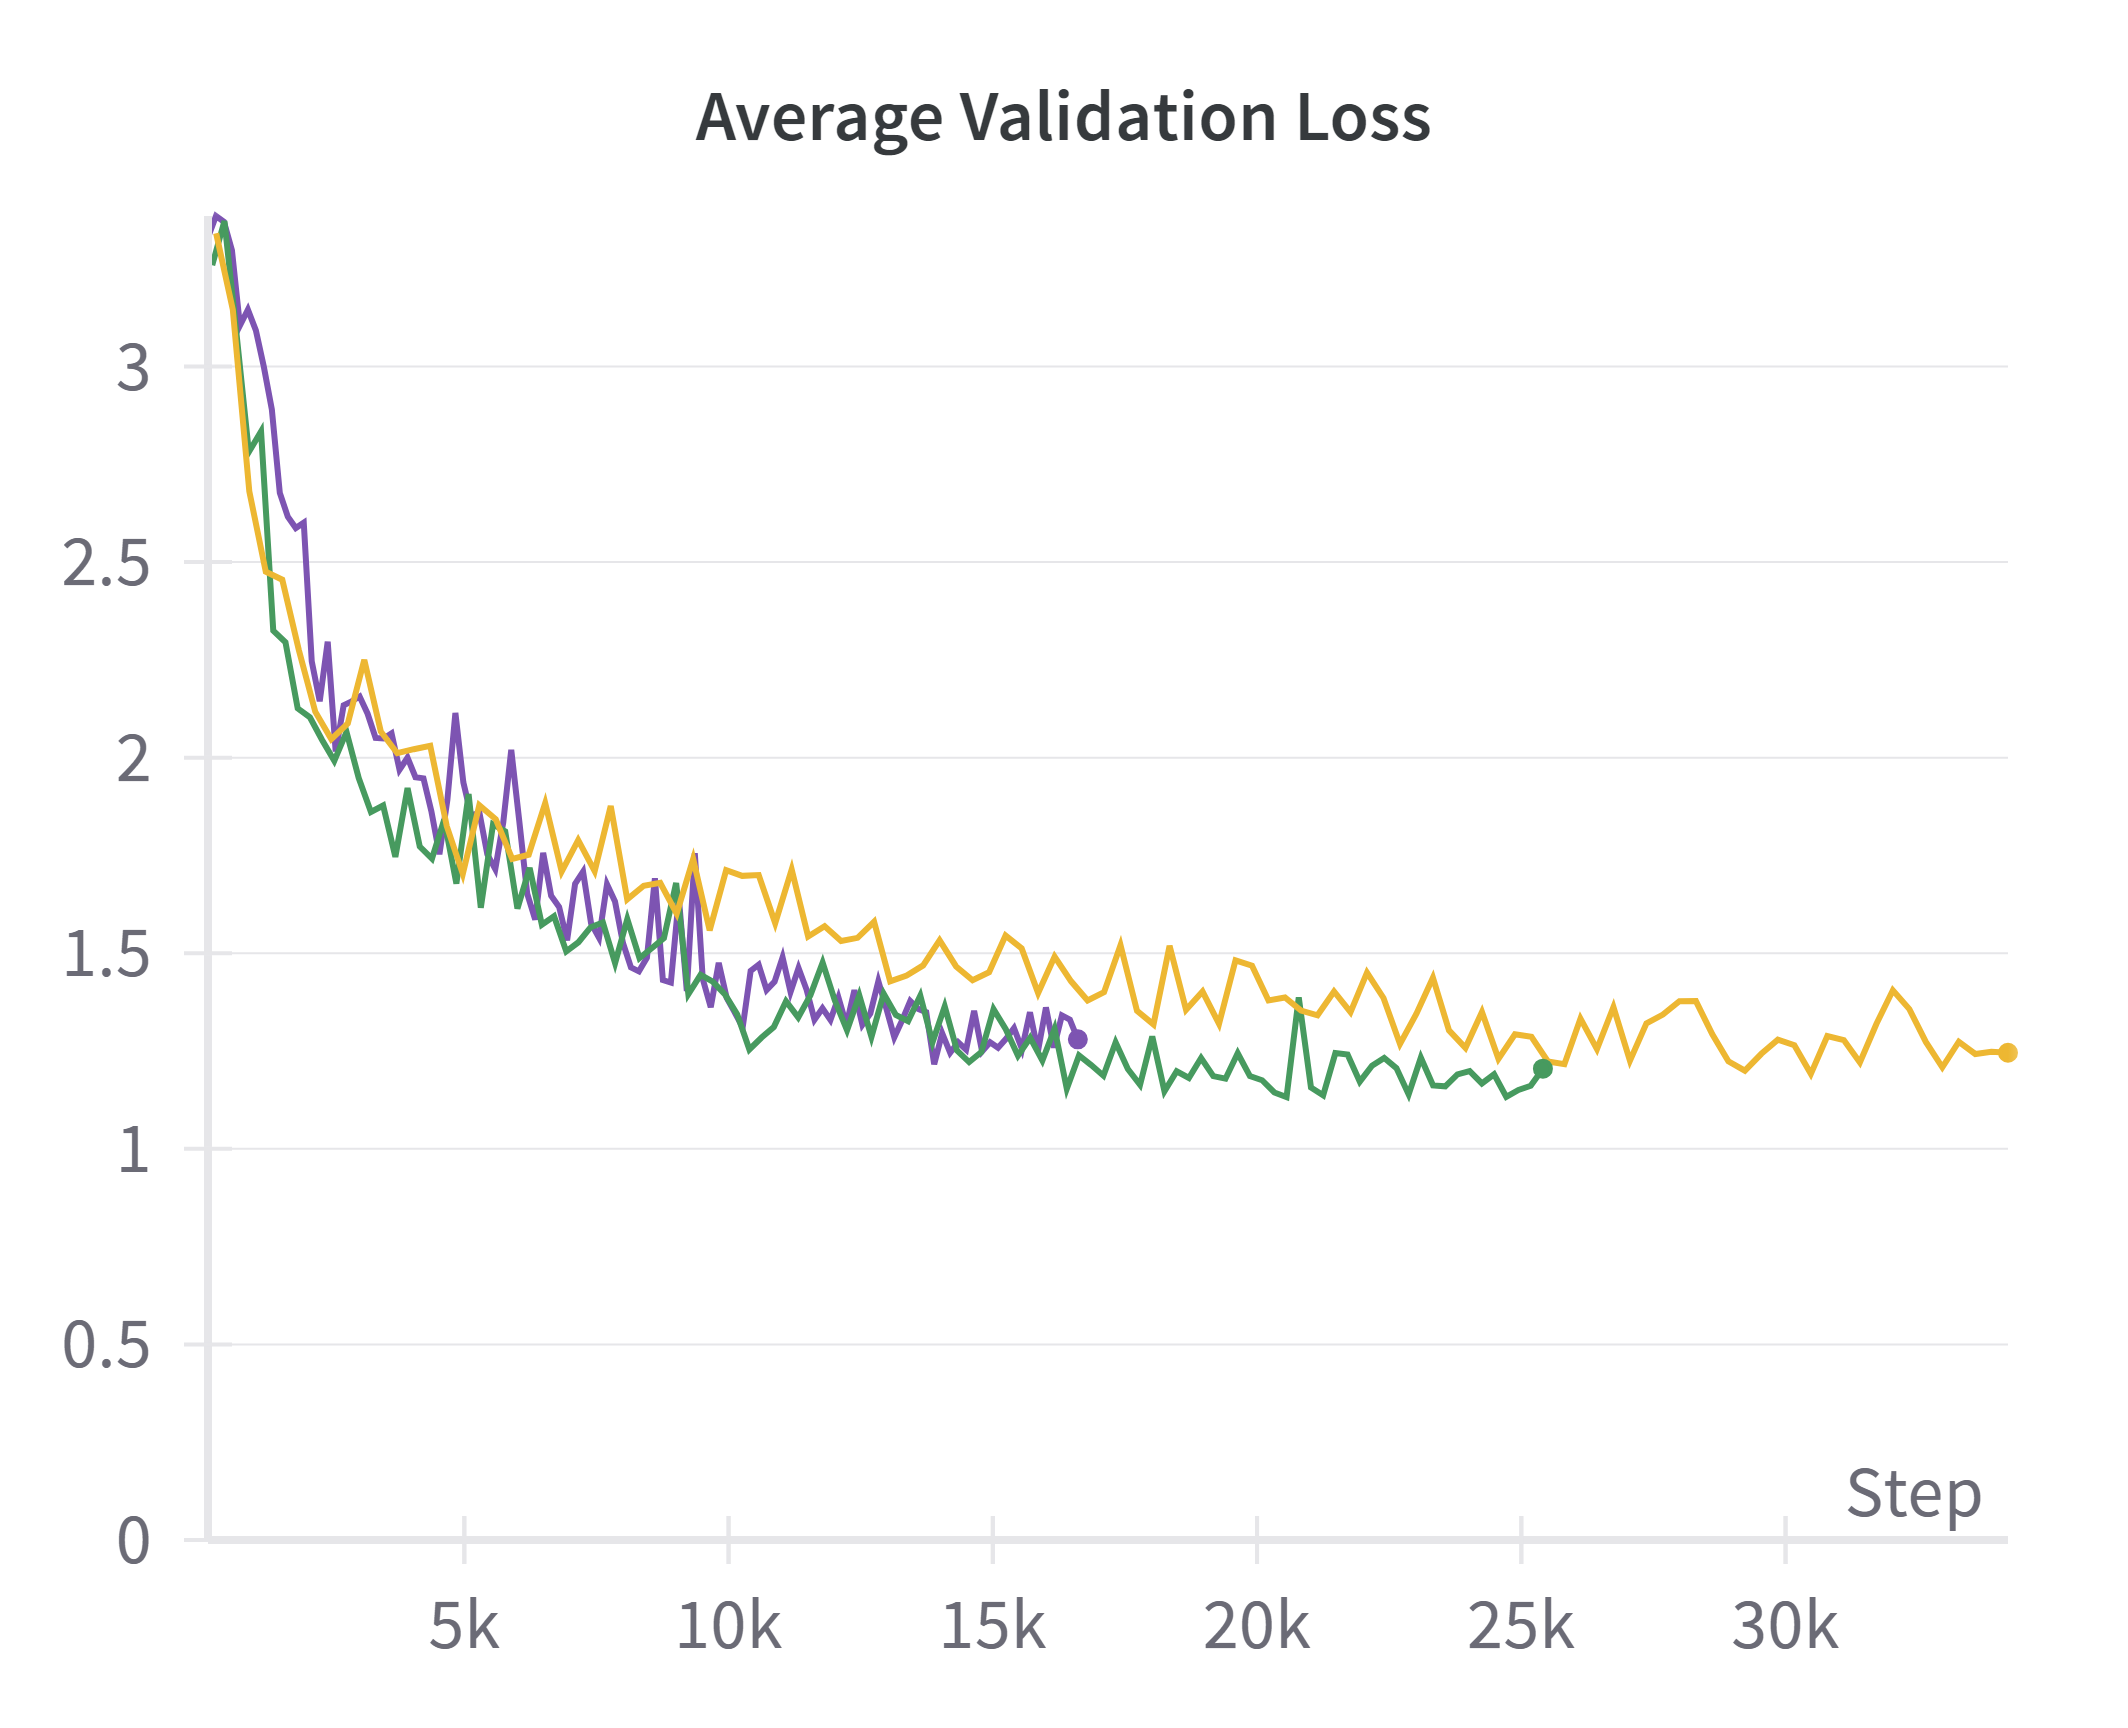
\includegraphics[width=0.5\textwidth]{figure_results_supcon-pre_avg-val-loss.png}
	\caption{Beispieltext}
	\label{fig:supcon-pre-loss}
\end{figure}

...

\subsection{Lineare Klassifikation} \label{sec:supcon-lin-results}

% Nur reale Daten
% Mit ID-Augmentationen
% Mit ID-Augmentationen und Contrastive Pre-Training mit OOD-Augmentationen
...

\begin{figure}
	\centering
	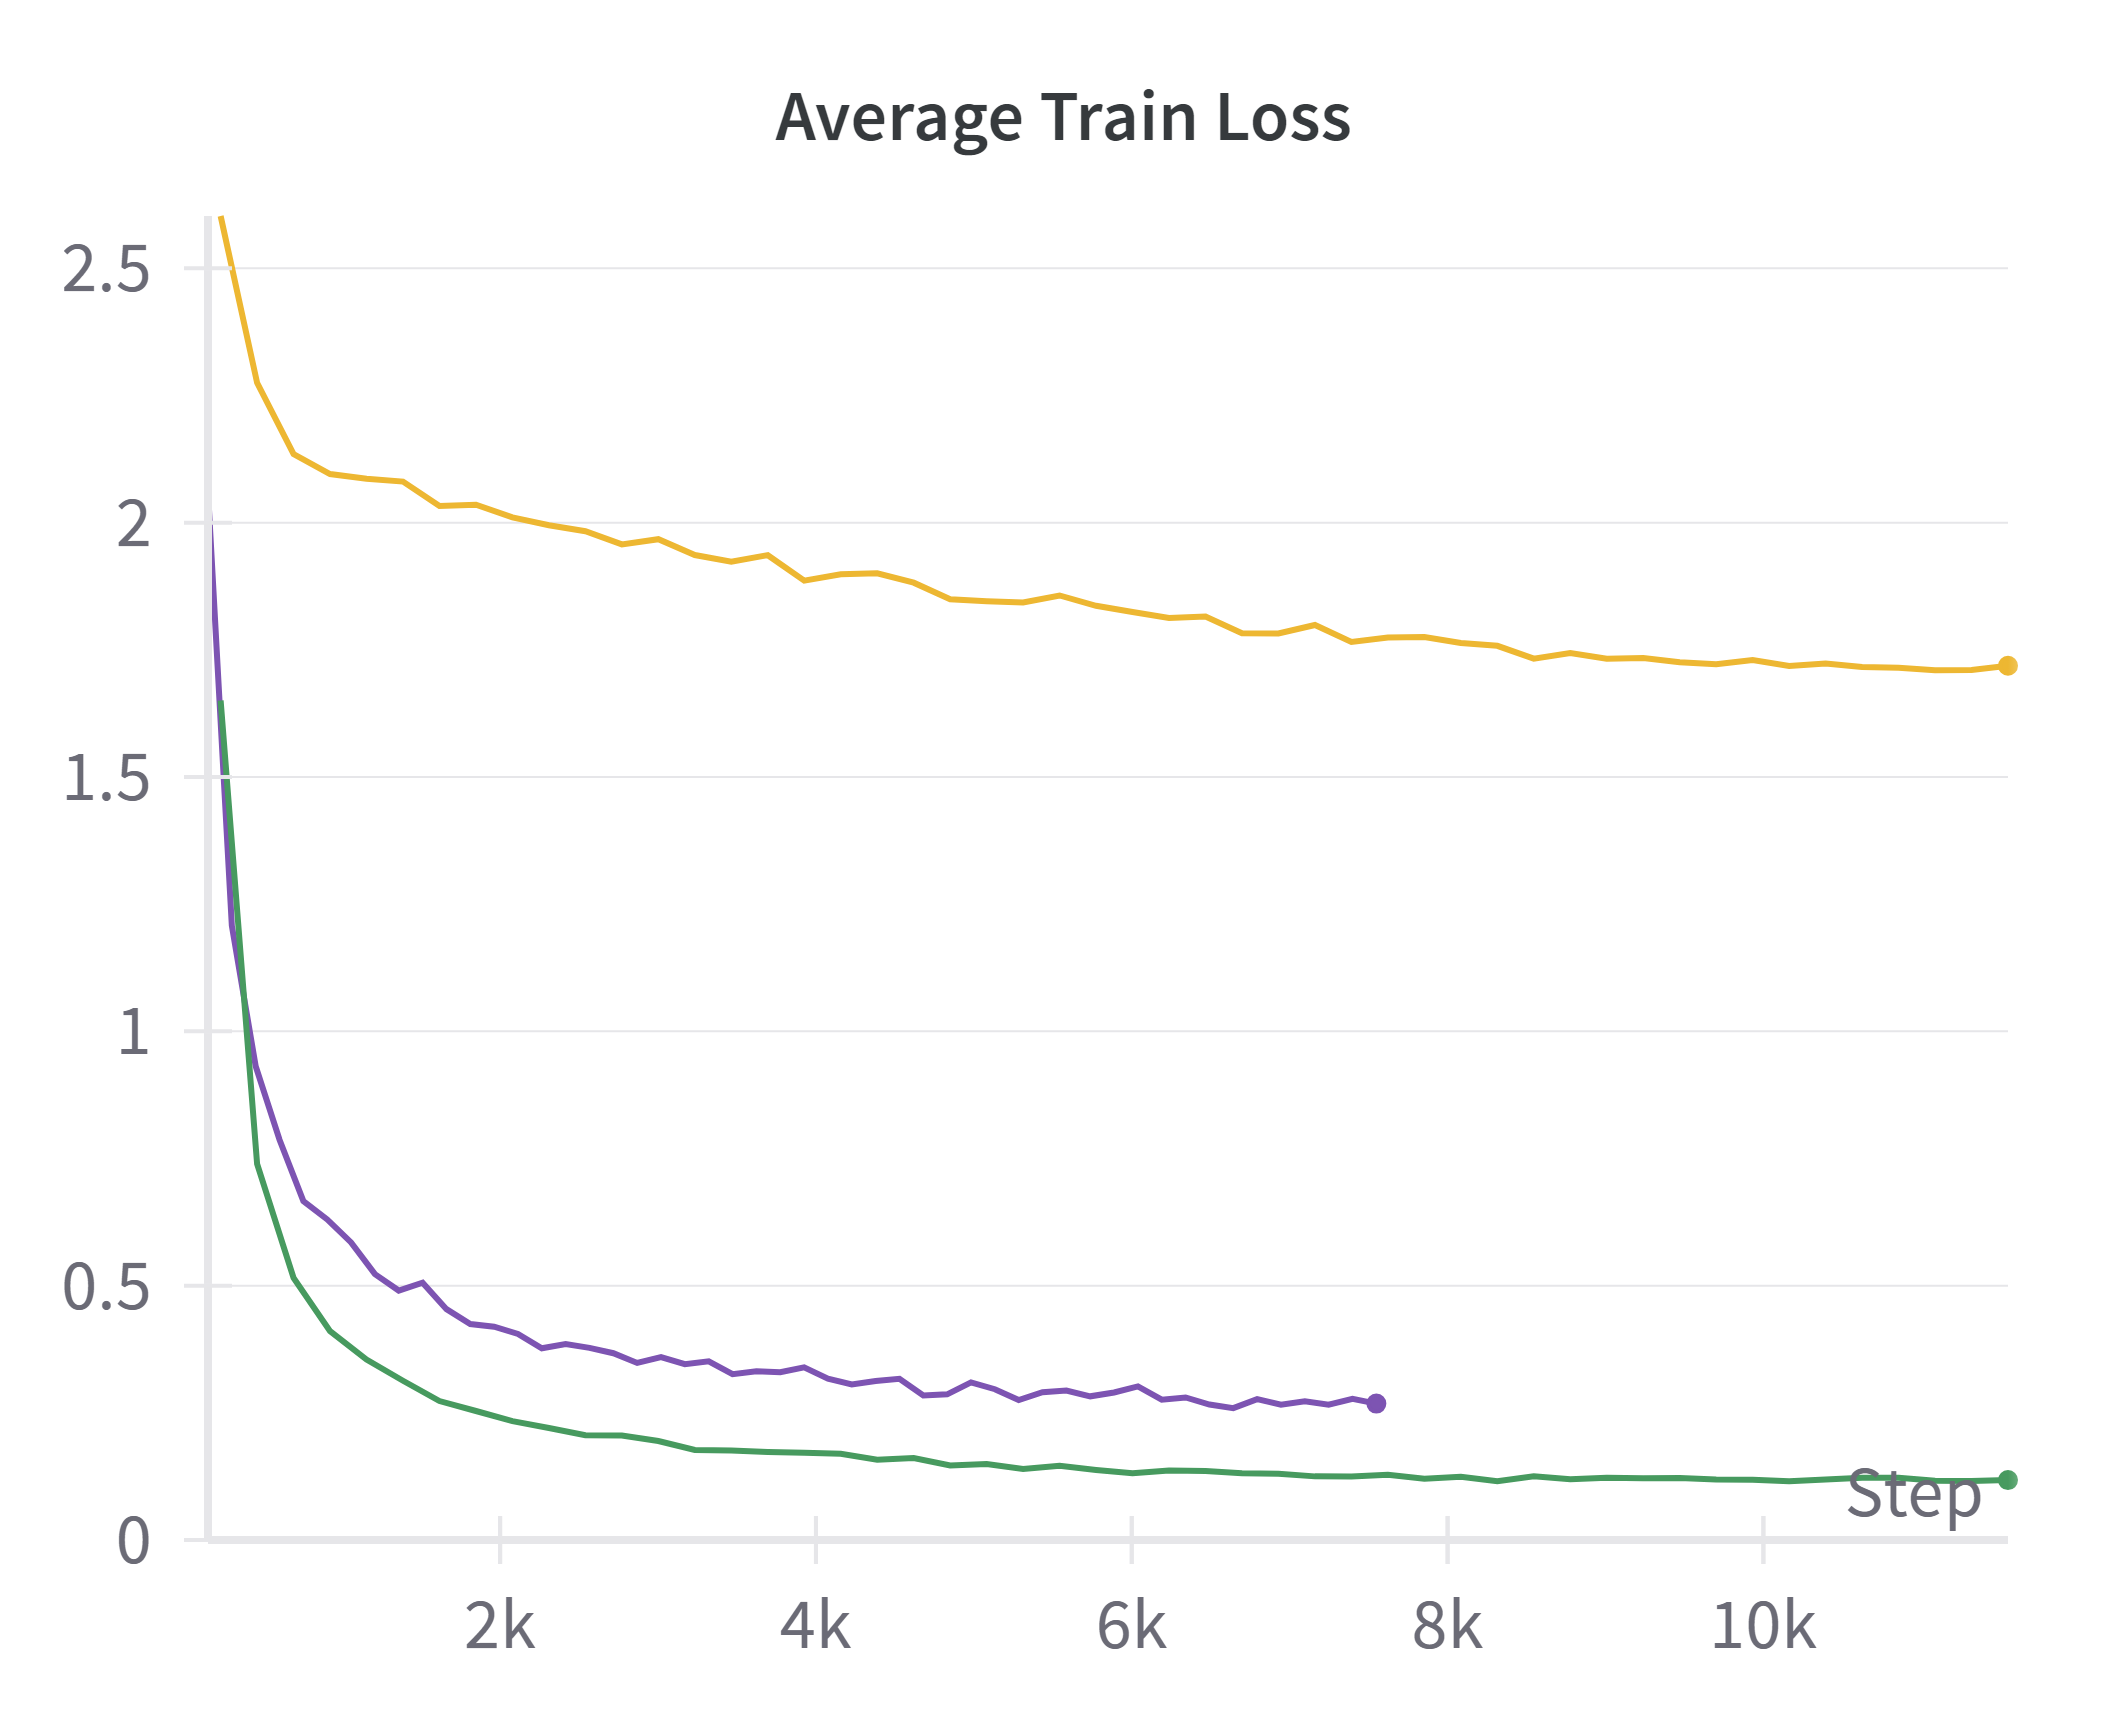
\includegraphics[width=0.5\textwidth]{figure_results_supcon-lin_avg-train-loss.png}%
	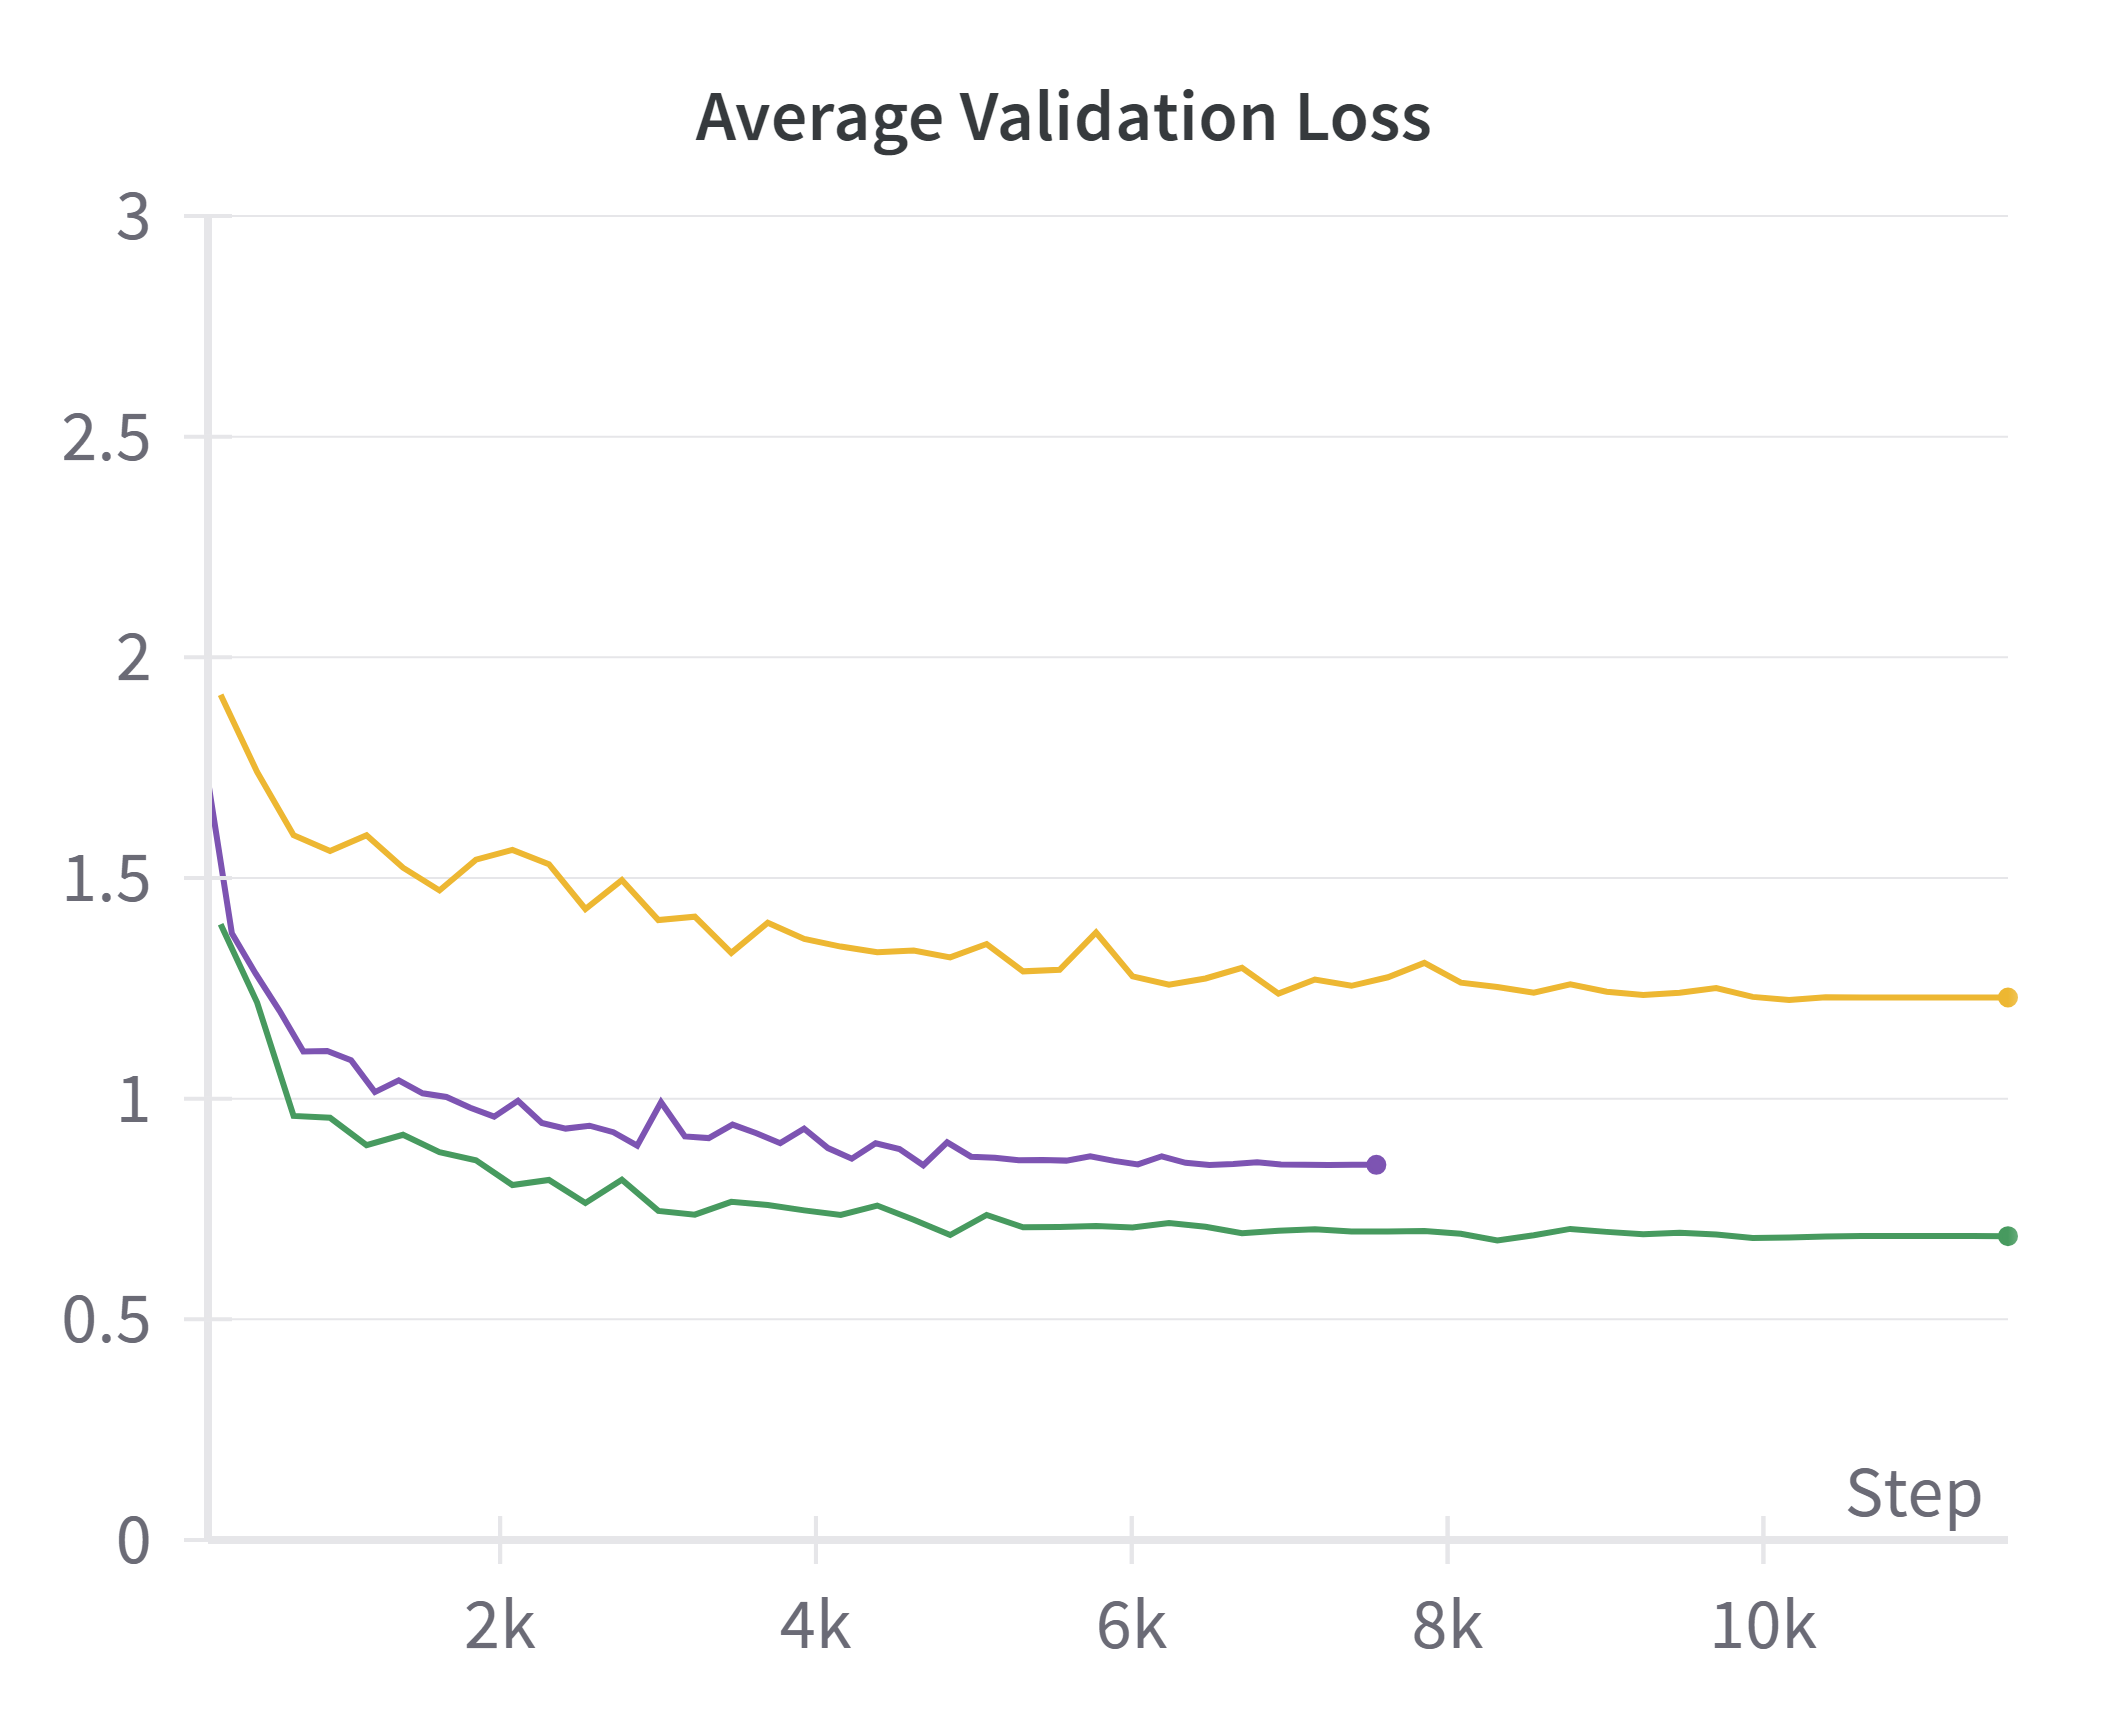
\includegraphics[width=0.5\textwidth]{figure_results_supcon-lin_avg-val-loss.png}
	\caption{Beispieltext 1}
	\label{fig:supcon-lin-loss}
\end{figure}
\begin{figure}
	\centering
	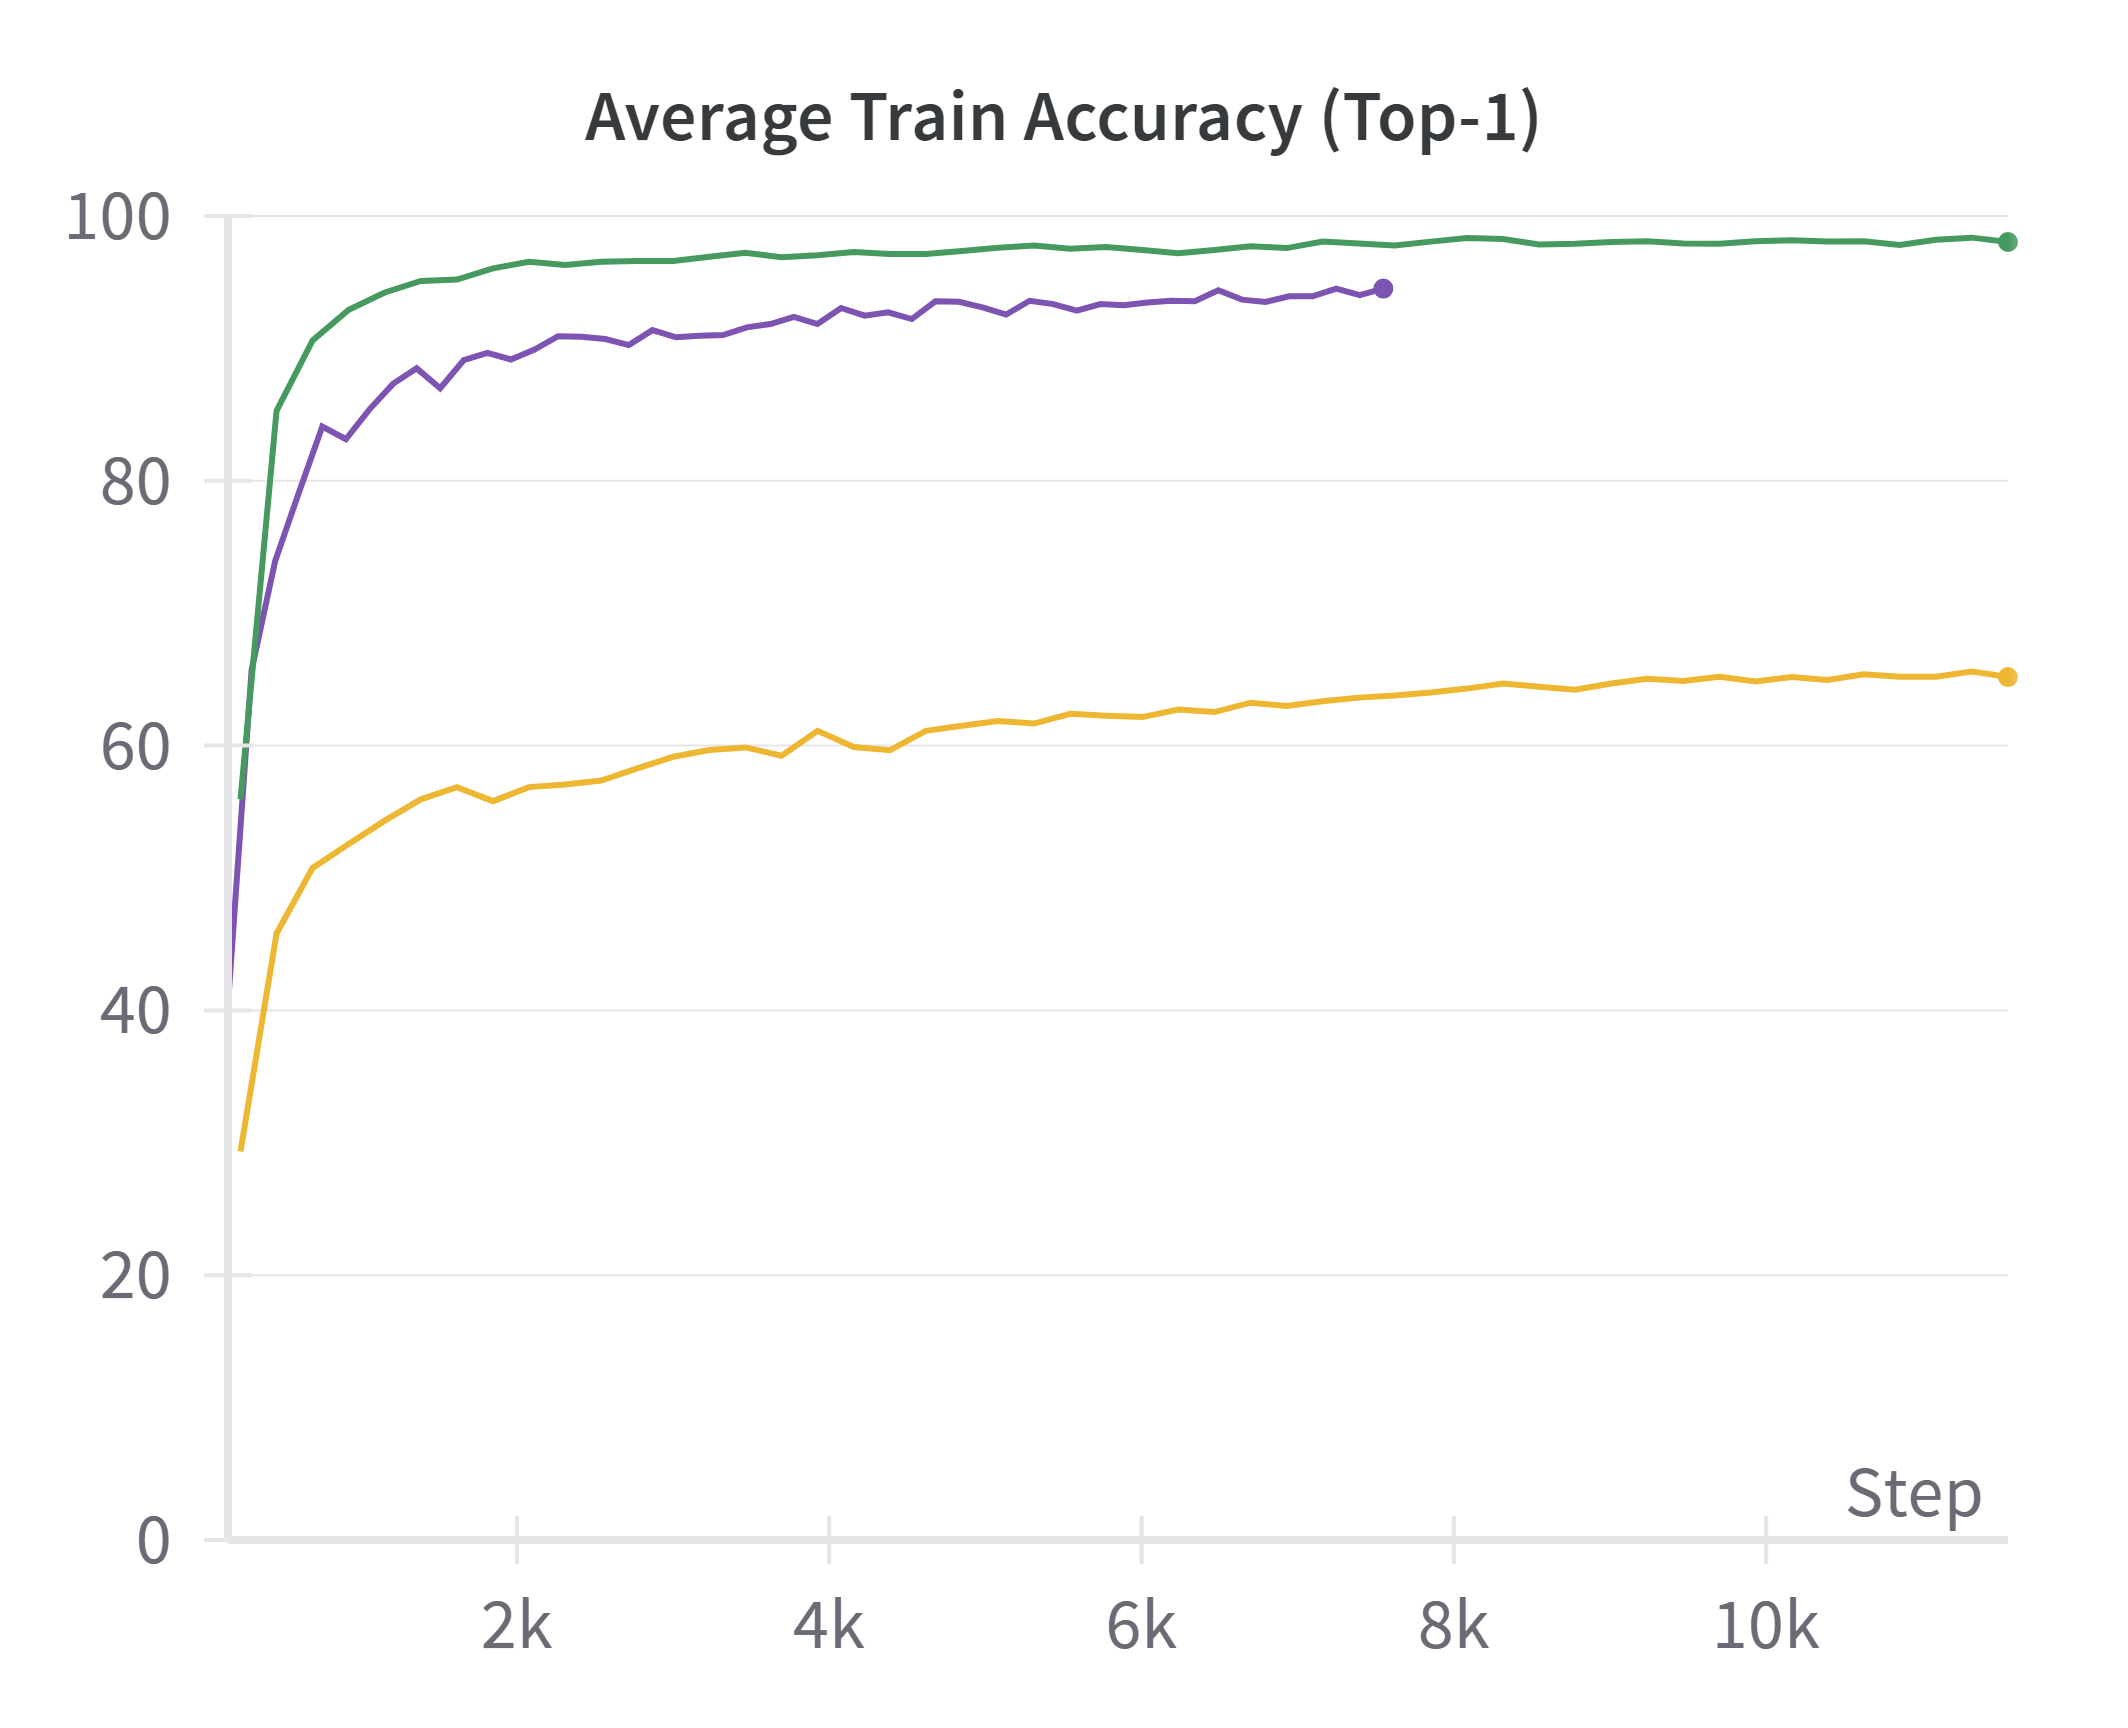
\includegraphics[width=0.5\textwidth]{figure_results_supcon-lin_avg-train-acc.png}%
	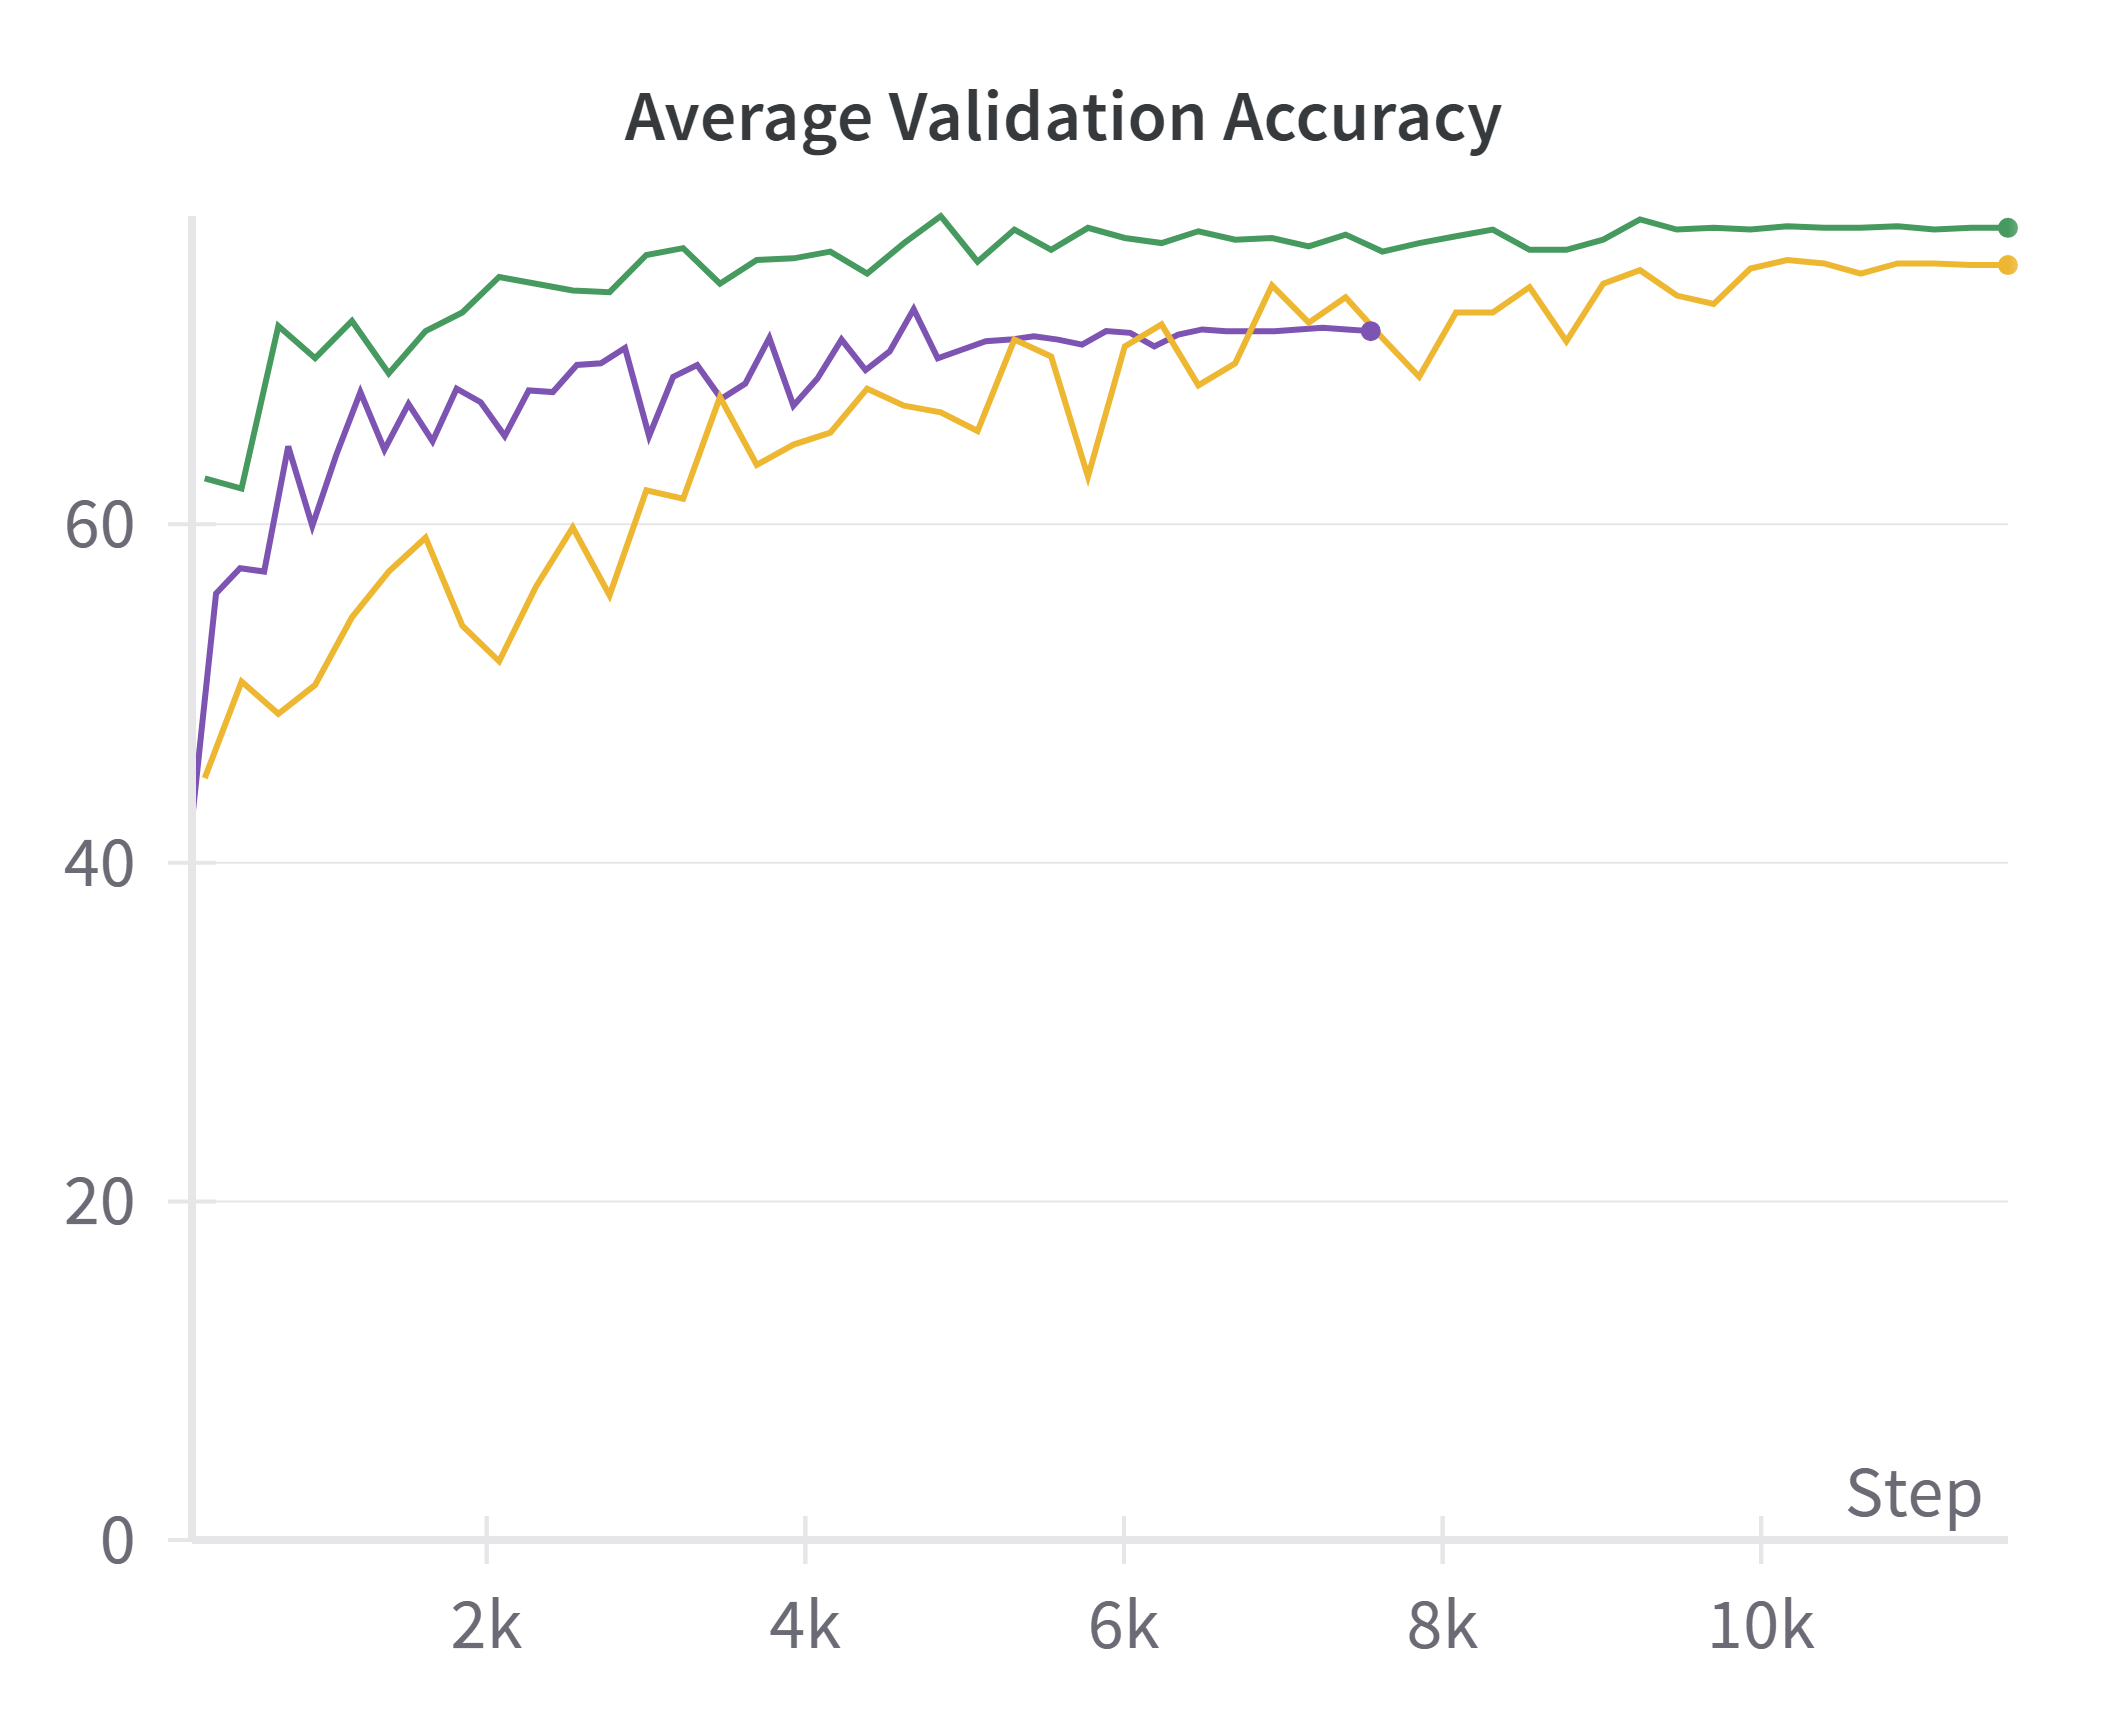
\includegraphics[width=0.5\textwidth]{figure_results_supcon-lin_avg-val-acc.png}
	\caption{Beispieltext 2}
	\label{fig:supcon-lin-acc}
\end{figure}
\begin{figure}
	\centering
	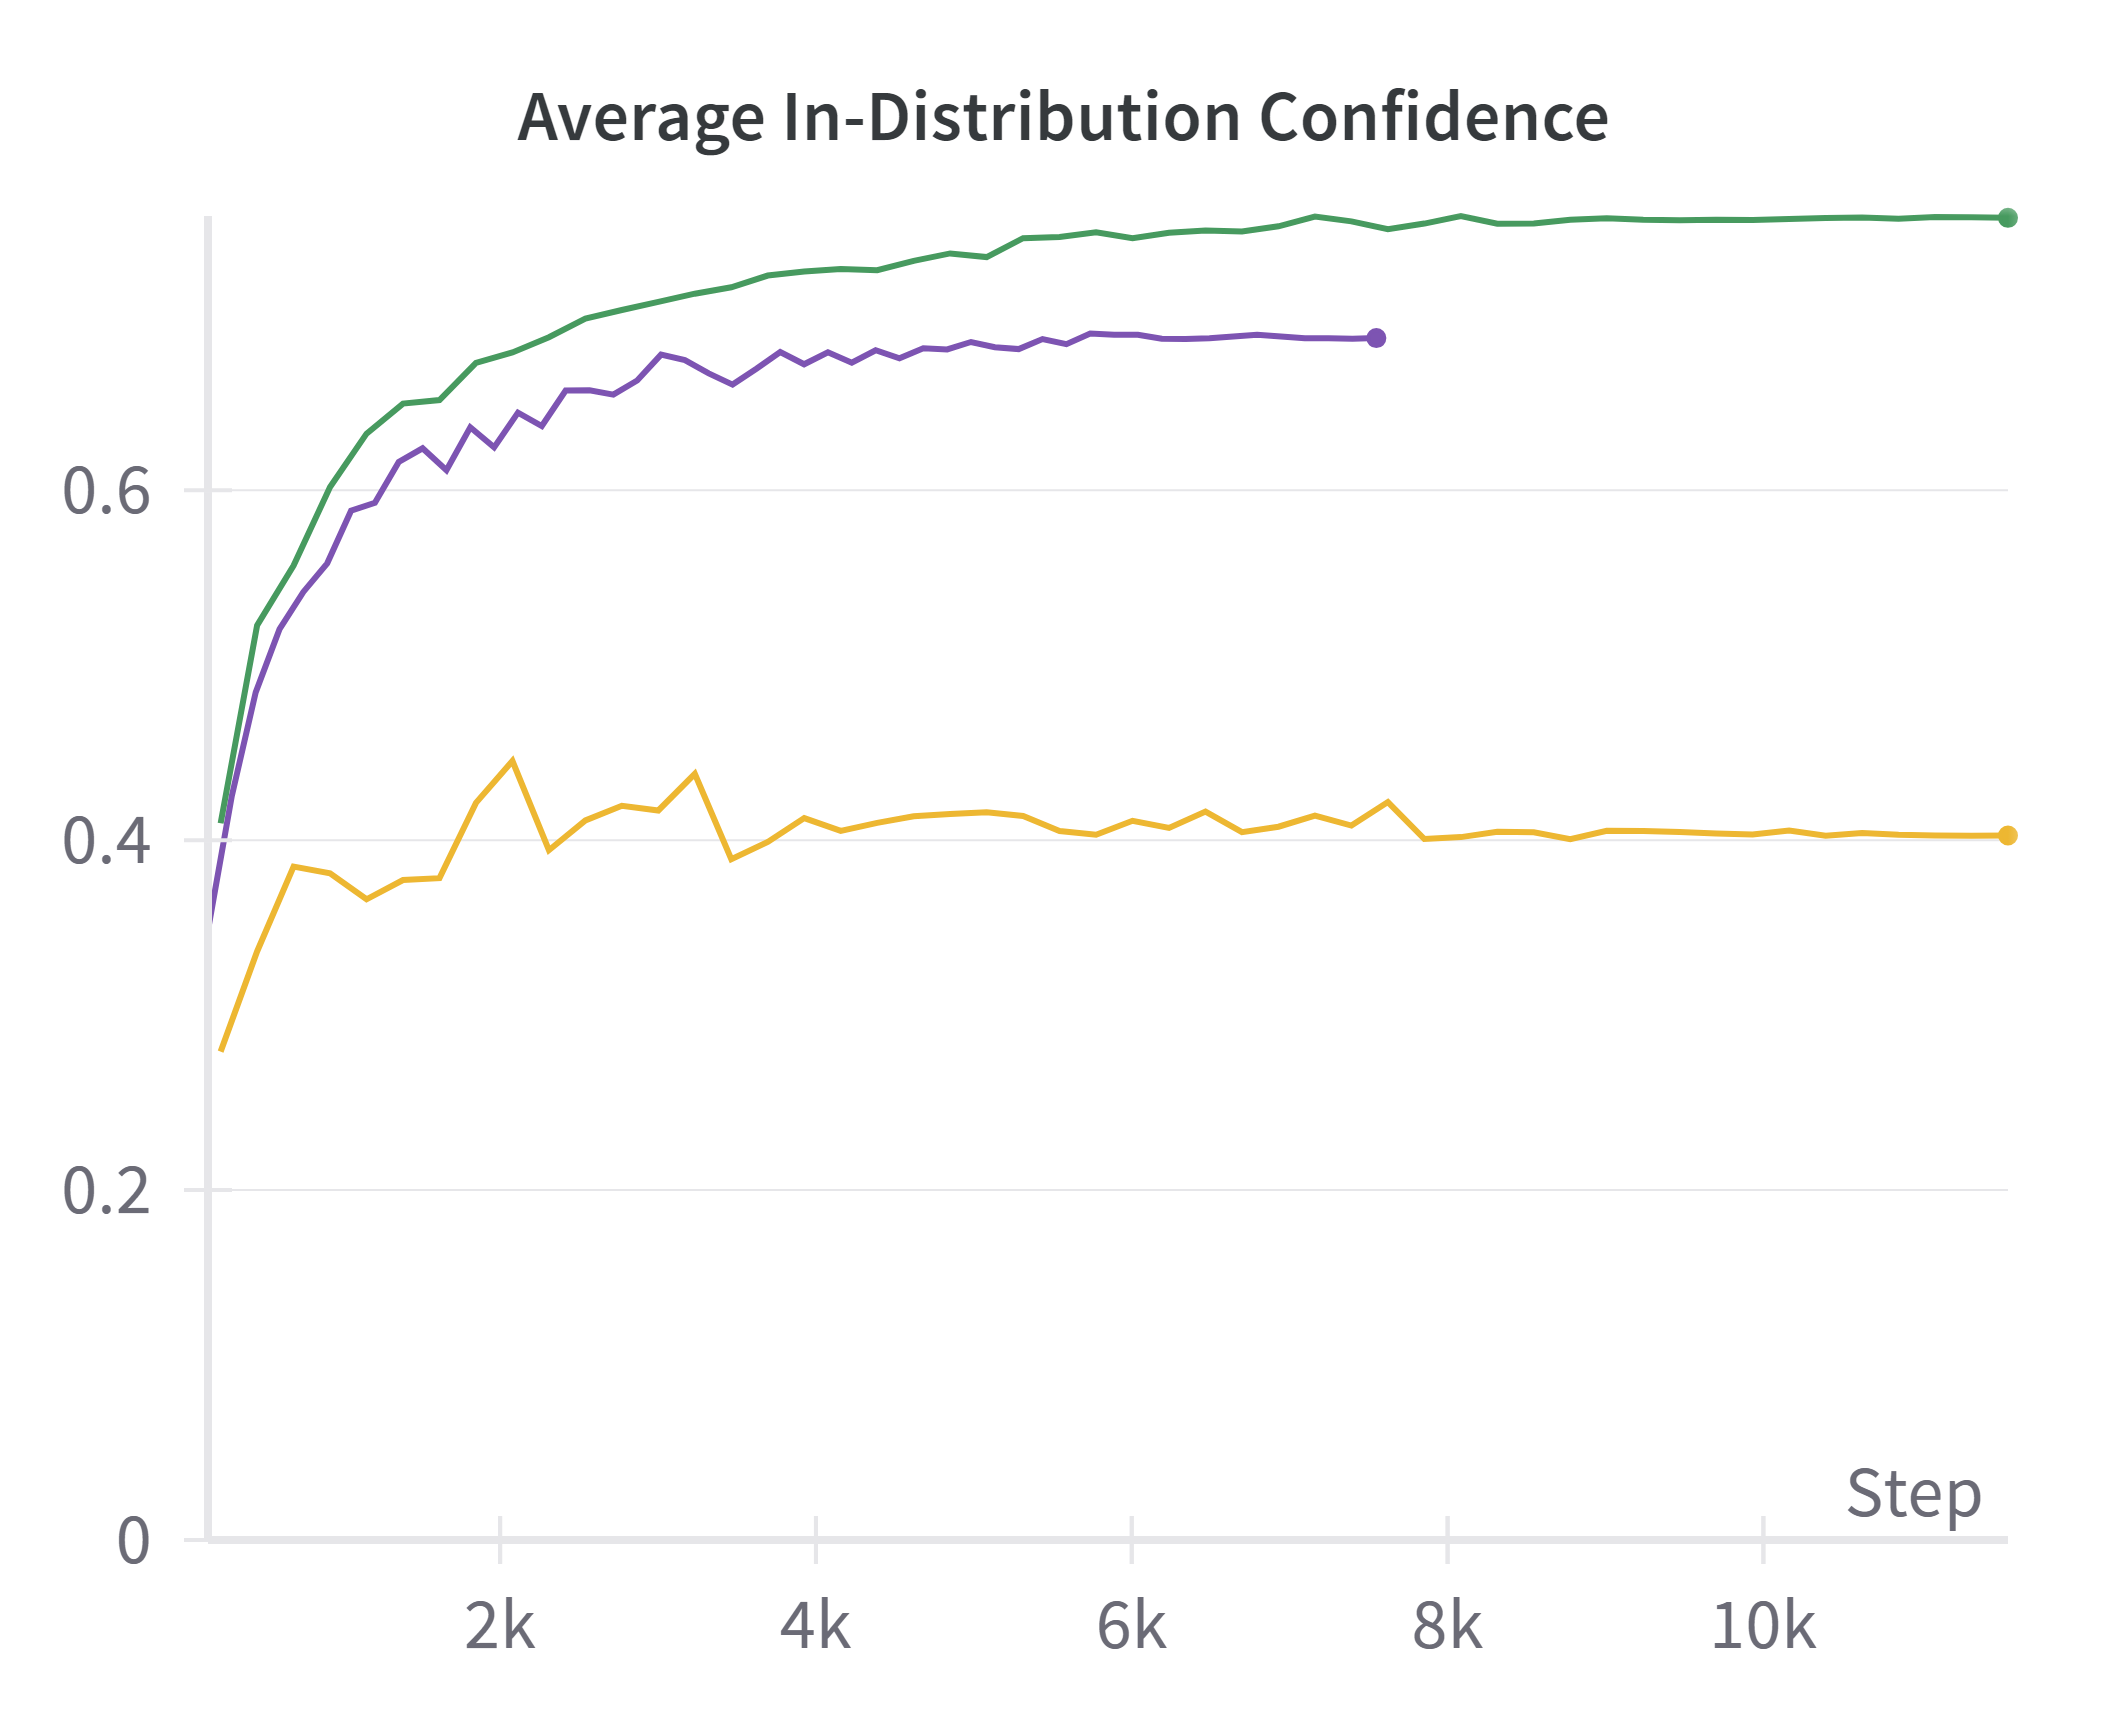
\includegraphics[width=0.5\textwidth]{figure_results_supcon-lin_avg-id-conf.png}%
	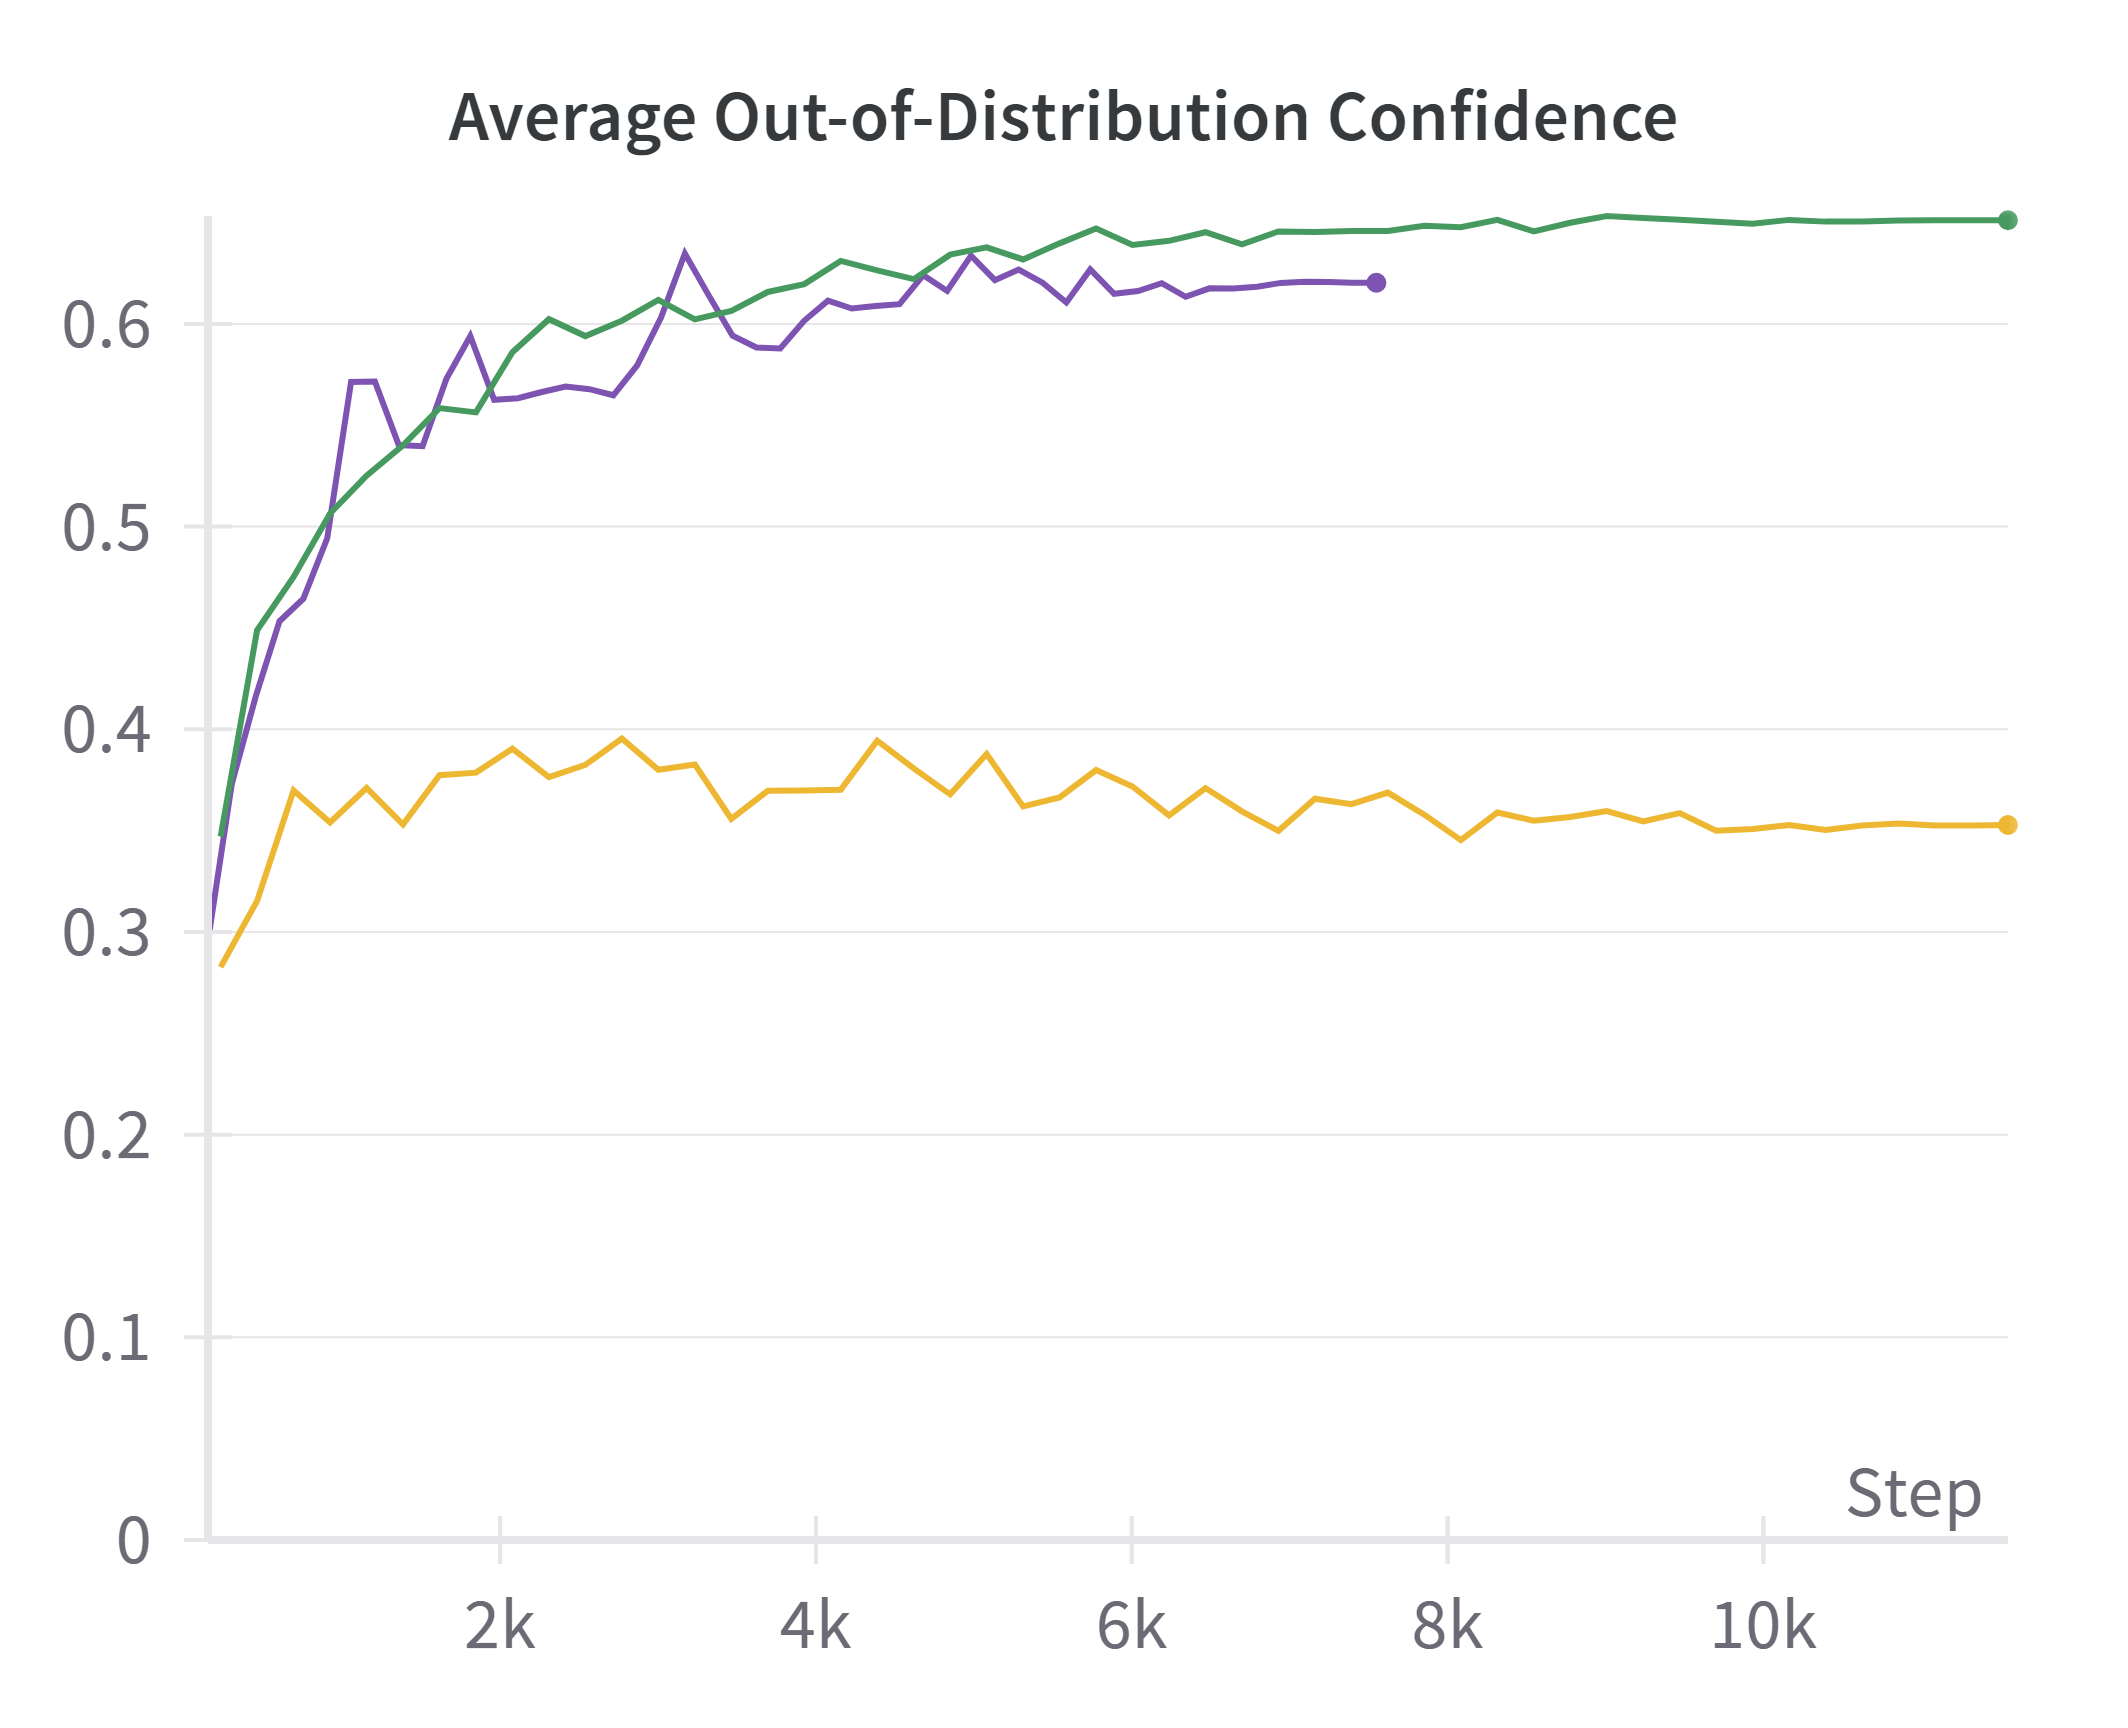
\includegraphics[width=0.5\textwidth]{figure_results_supcon-lin_avg-ood-conf.png}
	\caption{Beispieltext 3}
	\label{fig:supcon-lin-ood-detection}
\end{figure}

...

\begin{table}
	%\centering
	\caption{Testergebnisse der linearen Klassifikation.}
	\begin{tabular}{|c|c|c|}
		\hline
		\textbf{Versuch} & \textbf{Accuracy (\%)} & \textbf{ID-/OOD-Confidence (Differenz)} \\
		\hline
		1 & 71.4 & 0.69 / 0.62 (0.07) \\
		2 & 77.5 & 0.76 / 0.65 (0.11) \\
		3 & 75.3 & 0.40 / 0.35 (0.05) \\
		\hline
	\end{tabular}
	\label{tab:supcon-lin-results}
\end{table}

\section{Vergleich der Ergebnisse} \label{sec:results-comparison}

...

\subsection{Mit und ohne In-Distribution-Augmentationen} \label{sec:results-comparison-id}

...

\subsection{Mit und ohne Near Out-of-Distribution-Augmentationen} \label{sec:results-comparison-ood}

...
